\section{Demonstration}
\label{demo_section}

In this section, we demonstrate the use of GreenMeasurer in both calibration modes and for the two types of measurements it can perform while executing the recursive Fibonacci(55) implementation in C. We used this program as a simple example that generates enough computational load to produce stable and comparable energy measurements. Using smaller input values would lead to shorter executions, making the results more sensitive to background system activity and measurement noise.

The machine used for the demonstration was running Linux Ubuntu~22.04, equipped with an Intel(R) Core(TM) i7-8750H processor (6~cores, 12~threads, base clock 2.2~GHz, turbo speed 4.1~GHz), 16~GB of RAM and cache sizes of 384~KB (L1), 1.5~MB (L2) and 9~MB (L3).

All data used in this section can be found in the \texttt{paper\_data} folder of the repository. This includes CSV files containing the results, text files from the power cap and temperature calibrations, and Jupyter Notebook (\texttt{.ipynb}) files used to generate the graphs.

An important aspect of any energy measurement framework is the overhead it introduces during execution. GreenMeasurer performs measurements externally through system calls in C, avoiding modifications to the target program. To estimate the impact of this approach, we refer to the study by Pereira et~al.~\cite{PEREIRA2021102609}, which evaluated an earlier version of this framework. In their experiments, the energy readings obtained through system calls were compared to direct RAPL and jRAPL measurements within program source code. The observed differences were found to be insignificant, indicating that the overhead introduced by this external measurement mechanism is minimal. Although these results were obtained with a previous version, they suggest that the current GreenMeasurer implementation likely introduces negligible measurement overhead as well.


The first step is temperature calibration. To do this, we executed a \textit{sleep 60} command and measured the average temperature afterward. The resulting baseline temperature for subsequent executions was 43.8\textdegree C. Note that the file \texttt{cores\_temperature.txt} contains the complete output of the \textit{sensors} command, but the relevant information is in the last line ("\texttt{Average temperature: 43.8\textdegree C}").

Next, we performed the power cap calibration to determine the optimal power cap value. In this step, we aimed to identify the power cap at which the \textit{Package} power consumption is minimized. We tested power cap settings ranging from 2 W to 25 W using the Python implementation of the Fibonacci algorithm provided in the \texttt{Utils/} folder, with an input value of 40. During this process, we also configured three additional parameters: a time limit of 4~hours for each program execution, a CPU temperature variance threshold of 5\textdegree{}C and the number of repetitions for each program (4 runs).
 The standard output of this calibration, available in the file \texttt{powercap\_report.txt}, summarizes the results. Based on this analysis, we found that a power cap value of \textit{4~W} provides the most efficient balance. Therefore, all subsequent measurements were conducted using this setting. In the following subsections, we present the results for each type of measurement offered by GreenMeasurer. For this purpose, we used the \texttt{measure.sh} Bash script.

\subsection{Standard Measurements}
\label{stdM_results}

To demonstrate how GreenMeasurer can measure the energy consumption and execution time of a software system (referred to here as \textit{standard measurements}), we ran the Fibonacci algorithm in C with an input of 55, both without power capping and with a power cap of 4~W, repeating each configuration 10 times (\textit{n\_times = 10}), with a \textit{time\_out\_limit} of 4~hours and a CPU temperature variance threshold of 5\textdegree C, as defined during the power cap calibration process. Figure~\ref{fig:std} shows the RAPL energy components (\textit{Package}, \textit{Core}, \textit{DRAM} and \textit{GPU}) along with the runtime for all 10 measurements. We observe that applying a power cap reduces the energy consumption of all components but increases the runtime. This behavior was previously reported in~\cite{10.1145/3687997.3695638}, although in that study, energy consumption was measured only at the \textit{Package} level. Our primary goal here is to demonstrate that GreenMeasurer can measure energy components and runtime for software systems, so an in-depth analysis of these results is beyond the scope of this paper.

\begin{figure}[!ht]
    \centering
    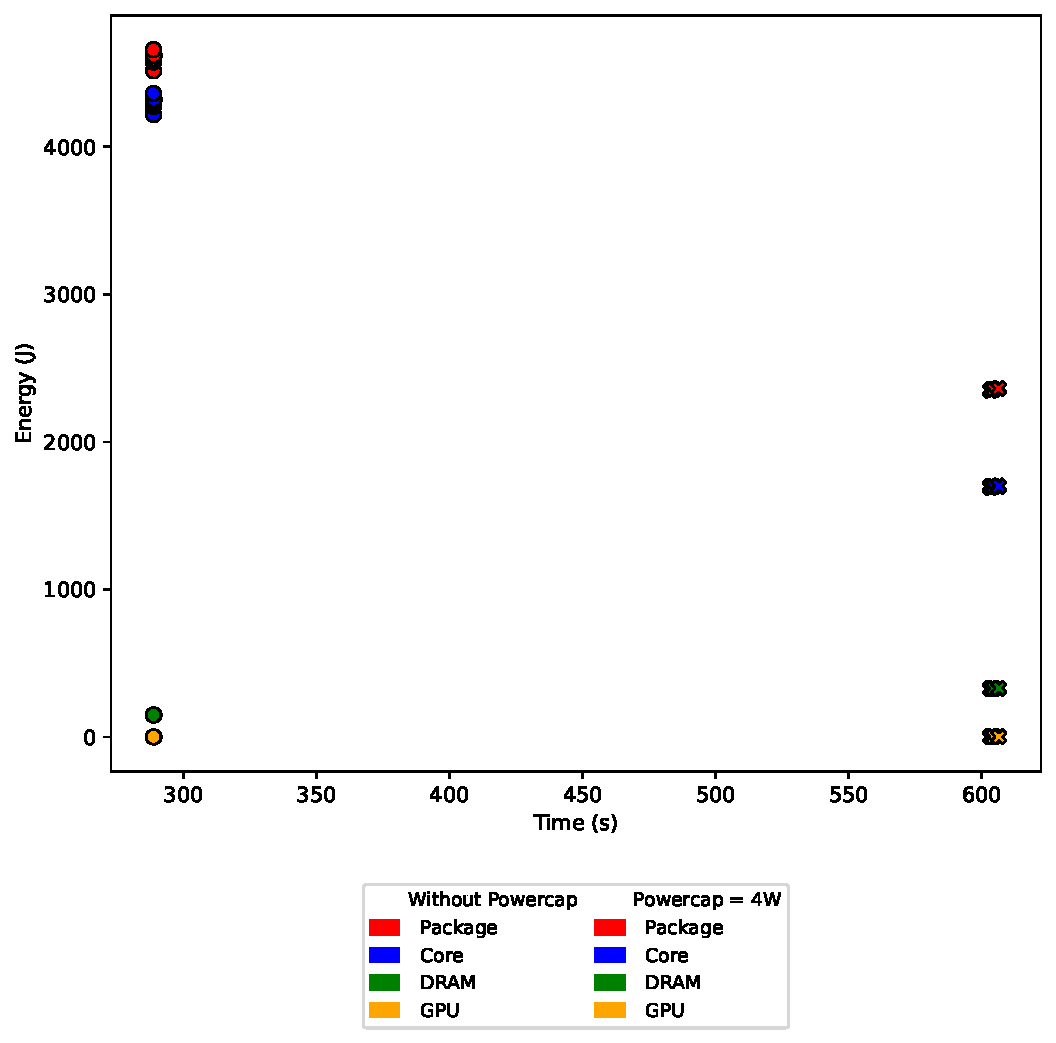
\includegraphics[width=1\linewidth]{images/results/std.pdf}
    \caption{Standard Results for Fibonacci(55) in C}
    \label{fig:std}
\end{figure}

\subsection{Over-Time Measurements}

In this type of measurement, we executed the same Fibonacci program in C using the parameters described in Section~\ref{stdM_results}, except for the number of executions (\textit{n\_times}), which ranged from 10 to 1 for demonstration purposes only. The experiments were conducted both with a 4~W power cap and without any power cap enabled. This setup allows us to compare the four energy counters under consideration throughout the program's execution. As shown in Figure~\ref{fig:Overtime_res}, the CPU temperature increases during execution without a power cap but decreases when the power cap is applied, which is consistent with the expected behavior due to power limitation. Furthermore, the total energy consumption decreases when the power cap is enabled, similarly to what was observed in Section~\ref{stdM_results}. As a suggestion for future researchers, increasing the measurement interval could provide a more detailed view of the results. Overall, these experiments demonstrate that GreenMeasurer can effectively measure both energy consumption and CPU temperature during the execution of a software system.

\begin{figure}[!ht]
    \centering
    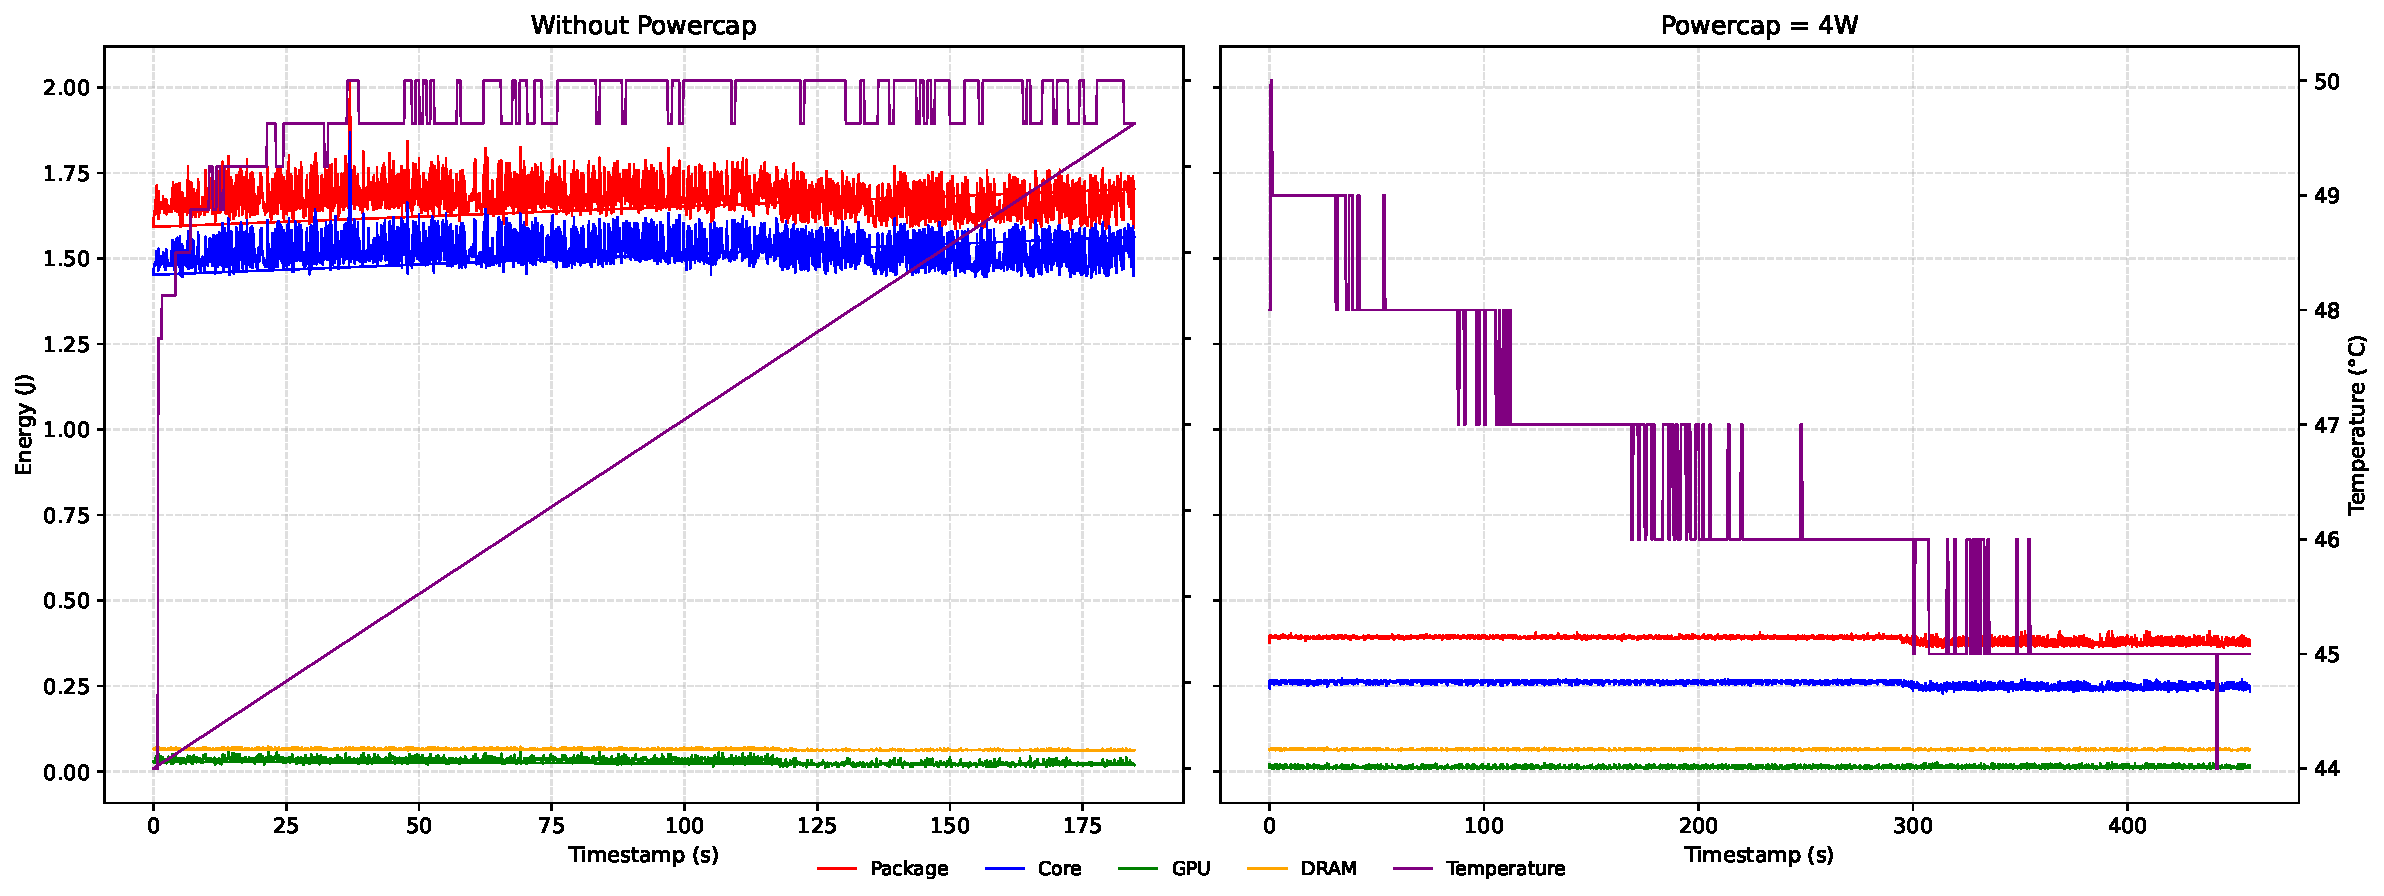
\includegraphics[width=1\linewidth]{images/results/overtime.pdf}
    \caption{Over-time results for Fibonacci(55) in C.}
    \label{fig:Overtime_res}
\end{figure}

\subsection{Evaluation Plan: Comparison with CodeCarbon and EnergiBridge}
\label{sec:eval_plan}

\textbf{[Planned; no results yet.]} The workload is a recursive Fibonacci implementation in Python (\texttt{Languages/Python/Fibonacci}), deterministic and CPU-bound, with an input long enough (several seconds) to make the counters meaningful; the C version can be added to show language independence. GreenMeasurer, EnergiBridge and CodeCarbon are run on the same machine with the same workload, input and number of repetitions (e.g., 30). CodeCarbon wraps the Python call, whereas GreenMeasurer and EnergiBridge run the command externally. The planned experiments are:

\begin{enumerate}
    \item \textit{Standard mode.} Mean, standard deviation and coefficient of variation of energy (J) and time (ms) per tool, with the same system state in all runs and statistical tests of the differences.
    \item \textit{Over-time mode.} Cumulative energy and derived power over time, compared with the time series of the other tools where available, and the final total compared with experiment 1.
    \item \textit{Tool overhead.} Energy and time of the workload with each tool versus without any tool, and of an idle period of the same length.
    \item \textit{Usability and extensibility.} Steps and configuration lines needed to measure the same workload, and the files and lines needed to add a backend (with no change to the core), summarized in a feature table.
    \item \textit{Portability} (depending on the available machines). Experiment 1 on systems with different CPUs, with and without an NVIDIA GPU, reporting which backends were detected and how unsupported ones were reported.
\end{enumerate}

Threats to validity: the counters measure hardware domains and not the process; the tools may read different domains (package, whole system or modelled values), so absolute differences must be explained and not assumed to be errors; and the results are limited to the tested machines. AMD CPUs are not covered.

